%%%%%%%%%%%%%%%%%%%%%%%%%%%%%%%%%%%%%%%%%
% baposter Landscape Poster
% LaTeX Template
% Version 1.0 (11/06/13)
%
% baposter Class Created by:
% Brian Amberg (baposter@brian-amberg.de)
%
% This template has been downloaded from:
% http://www.LaTeXTemplates.com
%
% License:
% CC BY-NC-SA 3.0 (http://creativecommons.org/licenses/by-nc-sa/3.0/)
%
%%%%%%%%%%%%%%%%%%%%%%%%%%%%%%%%%%%%%%%%%

%----------------------------------------------------------------------------------------
%	PACKAGES AND OTHER DOCUMENT CONFIGURATIONS
%----------------------------------------------------------------------------------------

\documentclass[landscape,a0paper,fontscale=0.285]{baposter} % Adjust the font scale/size here
\usepackage{url}
\usepackage{graphicx} % Required for including images
\graphicspath{{figures/}} % Directory in which figures are stored

\usepackage{amsmath} % For typesetting math
\usepackage{amssymb} % Adds new symbols to be used in math mode

\usepackage{booktabs} % Top and bottom rules for tables
\usepackage{enumitem} % Used to reduce itemize/enumerate spacing
\usepackage{palatino} % Use the Palatino font
\usepackage[font=small,labelfont=bf]{caption} % Required for specifying captions to tables and figures

\usepackage{multicol} % Required for multiple columns
\setlength{\columnsep}{1.5em} % Slightly increase the space between columns
\setlength{\columnseprule}{0mm} % No horizontal rule between columns

\usepackage{tikz} % Required for flow chart
\usetikzlibrary{shapes,arrows} % Tikz libraries required for the flow chart in the template

\newcommand{\compresslist}{ % Define a command to reduce spacing within itemize/enumerate environments, this is used right after \begin{itemize} or \begin{enumerate}
\setlength{\itemsep}{1pt}
\setlength{\parskip}{0pt}
\setlength{\parsep}{0pt}
}

\definecolor{lightblue}{rgb}{0.145,0.6666,1} % Defines the color used for content box headers

\begin{document}

\begin{poster}
{
headerborder=closed, % Adds a border around the header of content boxes
colspacing=1em, % Column spacing
bgColorOne=gray, % Background color for the gradient on the left side of the poster
bgColorTwo=white, % Background color for the gradient on the right side of the poster
borderColor=black, % Border color
headerColorOne=black, % Background color for the header in the content boxes (left side)
headerColorTwo=orange, % Background color for the header in the content boxes (right side)
headerFontColor=white, % Text color for the header text in the content boxes
boxColorOne=white, % Background color of the content boxes
textborder=roundedleft, % Format of the border around content boxes, can be: none, bars, coils, triangles, rectangle, rounded, roundedsmall, roundedright or faded
eyecatcher=true, % Set to false for ignoring the left logo in the title and move the title left
headerheight=0.1\textheight, % Height of the header
headershape=roundedright, % Specify the rounded corner in the content box headers, can be: rectangle, small-rounded, roundedright, roundedleft or rounded
headerfont=\Large\bf\textsc, % Large, bold and sans serif font in the headers of content boxes
%textfont={\setlength{\parindent}{1.5em}}, % Uncomment for paragraph indentation
linewidth=2pt % Width of the border lines around content boxes
}
%----------------------------------------------------------------------------------------
%	TITLE SECTION 
%----------------------------------------------------------------------------------------
%
{
\includegraphics[height=4em]{PS_HOR_RGB_2C.png}} % First university/lab logo on the left
{\bf\textsc{The Network of Foreign Direct Investment Flows}\vspace{0.5em}} % Poster title
{\textsc{J. Schoeneman, B. Zhu, \& B. Desmarais\\
  Pennsylvania State University}} % Author names and institution
{
\includegraphics[height=4em]{bdss.png}} % Second university/lab logo on the right

%----------------------------------------------------------------------------------------
%	OBJECTIVES
%----------------------------------------------------------------------------------------

\headerbox{Introduction}{name=objectives,column=0,row=0}{

The political economy of FDI literature has established several theoretical claims and empirical regularities regarding exogenous political and economic determinants of FDI inflows.  However, existing studies---based on monadic and to a lesser degree, dyadic regression models---overlook the complex dependencies that are likely to characterize the network. Recent developments in methodology for studying international relations show that the regression framework is typically inadequate for quantitatively modeling dyadic relational data, such as FDI flows. In this paper, we integrate hypotheses regarding exogenous determinants and novel hypotheses regarding structural dependencies into a comprehensive exponential random graph model (ERGM) for weighted networks.

\vspace{0.3em} % When there are two boxes, some whitespace may need to be added if the one on the right has more content
}

%----------------------------------------------------------------------------------------
%	INTRODUCTION
%----------------------------------------------------------------------------------------

\headerbox{Theory}{name=introduction,column=1,row=0,bottomaligned=objectives}{


}

%----------------------------------------------------------------------------------------
%	RESULTS
%----------------------------------------------------------------------------------------

\headerbox{Results}{name=results,column=2,span=2,row=0}{

\begin{multicols}{2}
\vspace{1em}
\begin{center}

\includegraphics[width=0.8\linewidth]{placeholder}
\captionof{figure}{Figure caption}
\end{center}


\end{multicols}

%------------------------------------------------

\begin{multicols}{2}
\vspace{1em}


\begin{center}

\includegraphics[width=0.8\linewidth]{placeholder}
\captionof{figure}{Figure caption}
\end{center}

\end{multicols}
}

%----------------------------------------------------------------------------------------
%	Acknowledgement
%----------------------------------------------------------------------------------------

\headerbox{Acknowledgement}{name=references,column=0,above=bottom}{

This material is based on work supported by the National Science Foundation under IGERT Grant DGE-1144860, Big Data Social Science.}

%----------------------------------------------------------------------------------------
%	REFERENCES
%----------------------------------------------------------------------------------------

\headerbox{References}{name=futureresearch,column=1,span=2,aligned=references,above=bottom}{ % This block is as tall as the references block

\begin{multicols}{2}
1. \\
2. \\
3. \\
4. \\
\end{multicols}
}

%----------------------------------------------------------------------------------------
%	CONTACT INFORMATION
%----------------------------------------------------------------------------------------

\headerbox{Contact Information}{name=contact,column=3,aligned=references,above=bottom}{ % This block is as tall as the references block

\begin{description}\compresslist
\item[Web] \url{https://github.com/desmarais-lab/FDI_IGERT_H}
\item[Email] jbs5686@psu.edu
\end{description}
}

%----------------------------------------------------------------------------------------
%	Network Plot
%----------------------------------------------------------------------------------------

\headerbox{Network Plots}{name=conclusion,column=2,span=2,row=0,below=results,above=references}{

\begin{multicols}{2}
\begin{center}
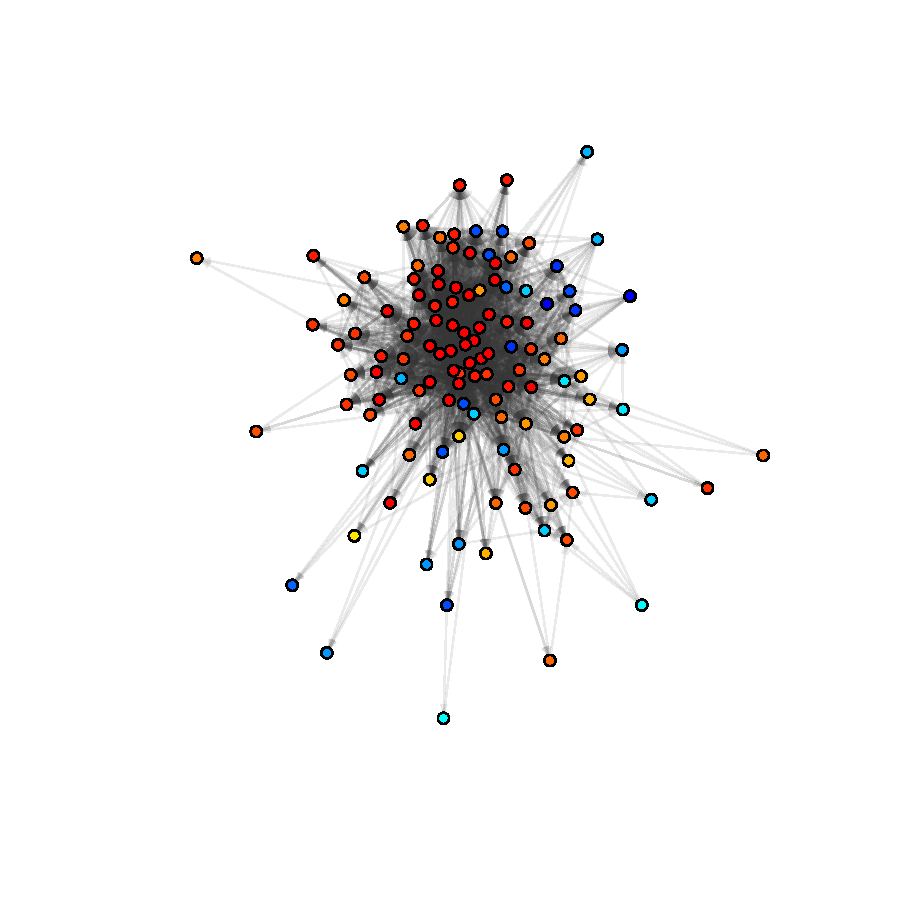
\includegraphics[width=0.8\linewidth]{fdiNet2011.pdf}
\captionof{figure}{Plot for 2011. Blue represents autocratic regimes and red represents democratic regimes}
\end{center}

%------------------------------------------------

\begin{itemize}\compresslist
\item Pellentesque eget orci eros. Fusce ultricies, tellus et pellentesque fringilla, ante massa luctus libero, quis tristique purus urna nec nibh. Phasellus fermentum rutrum elementum. Nam quis justo lectus.
\item Vestibulum sem ante, hendrerit a gravida ac, blandit quis magna.
\item Donec sem metus, facilisis at condimentum eget, vehicula ut massa. Morbi consequat, diam sed convallis tincidunt, arcu nunc.
\item Nunc at convallis urna. isus ante. Pellentesque condimentum dui. Etiam sagittis purus non tellus tempor volutpat. Donec et dui non massa tristique adipiscing.
\end{itemize}

\end{multicols}
}

%----------------------------------------------------------------------------------------
%	MATERIALS AND METHODS
%----------------------------------------------------------------------------------------

\headerbox{Data}{name=method,column=0,below=objectives,bottomaligned=conclusion}{ % This block's bottom aligns with the bottom of the conclusion block


}

%----------------------------------------------------------------------------------------
%	Count Model
%----------------------------------------------------------------------------------------

\headerbox{ERGM Count Model}{name=results2,column=1,below=objectives,bottomaligned=conclusion}{ % This block's bottom aligns with the bottom of the conclusion block

}

%----------------------------------------------------------------------------------------

\end{poster}

\end{document}